\documentclass{article}
\usepackage[utf8]{inputenc}
\usepackage{amsmath}
\usepackage{graphicx}
\usepackage{hyperref}
\parindent=0pt
\usepackage[a4paper, total={175mm, 252mm}]{geometry}
\usepackage[section]{placeins}
\usepackage{enumitem}
\usepackage{caption}
\usepackage{parskip}
\usepackage{multirow}

\title{PySpi for Persistent Sources}
\author{Möller, Julius}
\date{May 2023}

\begin{document}

\maketitle


\tableofcontents

\pagebreak


\section{General Procedure} \label{General Procedure}
In contrast to previous approaches to working with INTEGRAL SPI, this method does not attempt to fit the background via physical models, and instead uses a profile likelihood to eliminate its effect in the source model fit. The underlying assumption that allows this to work is that background count rates in each energy bin remain constant for temporally and spatially near SPI Science Windows (SCWs). Here we distinguish between source counts, which describe all detected events directly originating from astronomical objects considered in our source model, and background counts, which describe all other detector events.

This works in the following way: once we have split our set of SCWs into clusters within which we claim the assumption of constant background to be true and have defined a source model, a likelihood value can be calculated for each energy bin of each detector in each cluster. If one energy bin of one detector in one SCW with measuring time $t$ has a source count rate $s$ and a background count rate $b$, the probability $P$ of measuring $C$ counts follows a Poisson distribution:
\begin{equation}
    P(C \vert b, s, t) = \frac{\left( t \left( b + s \right) \right) ^C \text{exp}\left( -t \left( b+s\right)\right)}{C!}
\end{equation}

Equivalent energy bins in the same cluster are assumed to have the same background count rate $b$, so that the probability of measuring $C_1$ counts in one SCW and $C_2$ counts in another SCW is simply:

\begin{equation}
    P(C_1, C_2 \vert b, s_1, t_1, s_2, t_2) = P(C_1 \vert b, s_1, t_1) \cdot P(C_2 \vert b, s_2, t_2)
\end{equation}

The likelihood $\mathcal{L}$ for any energy bin of a detector within a cluster depends on all equivalent energy bins in that cluster, i.e. one term for each SCW in the cluster. If we have cluster of size two, the likelihood is described by:

\begin{equation}\label{log likelihood}
    \text{ln}\mathcal{L}(C_1, C_2, t_1, t_2\vert b, s_1 s_2) = \text{ln}P(C_1 \vert b, s_1, t_1) + \text{ln}P(C_2 \vert b, s_2, t_2)
\end{equation}

This expression allows us to solve for the probability distribution of $b$. A full and mathematically correct treatment of the background parameter $b$ turns out to be very cumbersome with only marginal benefits. Hence, the profile likelihood is used by simply solving for the background count rate value $b_M$ which maximizes the likelihood. This is easily done by setting the derivative of equation \ref{log likelihood} to zero and solving for $b$. For a cluster size of two one finds:
\begin{equation}
    b_M = \frac{1}{2} \left[ \frac{C_t}{t_t} - s_t + \sqrt{\left( \frac{C_t}{t_t} - s_t\right)^2 + 4 \left( \frac{C_1s_2+C_2s_1}{t_t}-s_1s_2\right)}\right]
\end{equation}
where $C_t=C_1+C_2$, $s_t=s_1+s_2$, and $t_t=t_1+t_2$. Using this maximum likelihood background $b_M$ finally allows us to compute a likelihood value that is only dependent on the measured counts and the source model:
\begin{equation}
    \text{ln}\mathcal{L}(C_1, C_2, b_M, t_1, t_2 \vert s_1, s_2) = \text{ln}P(C_1 \vert b_M, s_1, t_1) + \text{ln}P(C_2 \vert b_M, s_2, t_2)
\end{equation}
The process for clusters with sizes larger than two is analogous. One such likelihood value exists for every energy bin of every detector in every cluster, such that the total likelihood value for any given source model is simply the sum of the logarithmic likelihoods over all energy bins, detectors, and clusters. Thus the source model may be fitted to the count data by applying an algorithm to maximize the likelihood.


\section{Spimodfit Procedure}
In order to be able to compare the results obtained using PySpi and the method described above, spimodfit will be used with the same dataset. For the sake of limiting sources of potential errors, the procedure for obtaining results using spimodfit will be described in more detail than might otherwise be deemed necessary. In general, the  \href{https://www-cms.mpe.mpg.de/gamma/instruments/integral/www/}{spimodfit cookbook found here} was followed very closely. In all of the following sections only the SE Data was used by Spimodfit with an energy up to 600keV, compared to a possible 2MeV in the data used by Pyspi. 

\subsection{Fitting the Crab Nebula} \label{Spimodfit crab steps}

\begin{enumerate}
    \item On the ga05us.mpe.mpg.de PC, head into the directory:
    
    \verb|/home/jmoeller/cookbook/SPI_cookbook/examples/Crab|

    \item \label{scw select} In the file \verb|spiselectscw.cookbook_dataset_02_0020-0600keV_SE.par| specify which revolution(s) is to be used via the \verb|fits_revolutions_list| and \verb|revolutions_cond_value| parameters. Run the script:
    
    \verb|./submit-spiselectscw_ga05us.sh cookbook_dataset_02_0020-0600keV_SE &|

    \item \label{step background} In the file \verb|background_model_SE_02.pro| change the parameters \verb|spidir|, \verb|scw_file|, and \verb|bgdir| to point towards the correct directories in the newly created directory \verb|cookbook_dataset_02_0020-0600keV_SE|. Run this script: 
    
    \verb|idl idl-startup.pro background_model_SE_02.pro|

    \item \label{Source directory} In the file \verb|spimodfit.fit_Crab_SE_02.par| change the parameters \verb|counts_input_file|, \verb|pointing_input_file|, \verb|ebounds_input_file|, \verb|deadtime-dol|, \verb|gti-dol|, and \verb|background_input_file| to point to the correct directories. Furthermore, specify the source catalogue directory:
    
    \verb|source-cat-dol,s,h,"/home/jmoeller/cookbook/SPI_cookbook/cats/cat_crab.fits.gz"|

    Leave everything else untouched and run the script:

    \verb|./submit-spimodfit_v3.2_ga05us.sh fit_Crab_SE_02 clobber &|

    \item \label{Spectrum file} Inside the directory \verb|fit_Crab_SE_02| run the script \verb|./spimodfit_rmfgen.csh|. Back in the previous directory, edit the parameters \verb|response_file| and \verb|spectrum_file_01| in the file \verb|adjust4threeML_SE_02.pro| to point at the correct directories, and run the script:
    
    \verb|idl idl-startup.pro adjust4threeML_SE_02.pro|

    \item For convenience, transfer the files \verb|specra_Crab.fits| and \verb|spectral_response.rmf.fits| onto the local machine. Here the script found in
    
    \verb|/home/jmoeller/cookbook/SPI_cookbook/spectral_analysis/3ml_fit_Crab_SE.py|
    
    is used extract the fit parameters, where the source model and active measurements (i.e. energy range) can be changed as pleased.
\end{enumerate}


\subsection{Fitting other Sources}
If we want to fit another source instead of the Crab, the following changes are made to the previously described steps:

\begin{enumerate}
    \item Access the SPI source catalogue: \verb|/home/jmoeller/cookbook/SPI_cookbook/cats/spi_cat.fits.gz|
    \item Create a new file with only one (or more, depending on how many sources we want to fit) row from the source catalogue, representing one source. Edit the entries \verb|RA_OBJ|, \verb|DEC_OBJ|, and \verb|NAME| to the coordinates and name of the new source. Other entries in the row are not used and irrelevant for the fit.
    \item Place the new file in the same directory as the original catalogue.
    
    Now repeat steps from section \ref{Spimodfit crab steps} with the following differences:
    \item In step \ref{scw select} from section \ref{Spimodfit crab steps} also change the parameters 
    
    \verb|select_PtgX_masks_chi_list_1| and \verb|select_PtgX_masks_psi_list_1| 
    
    to the coordinates of the new source. Note that these are galactic coordinates.
    \item In step \ref{Source directory} from section \ref{Spimodfit crab steps} change \verb|source-cat-dol| to instead point to the new source file.
    \item The new spectrum output file will be names according to the new source name, which has to be reflected in the parameter \verb|spectrum_file_01| from step \ref{Spectrum file} in section \ref{Spimodfit crab steps}.
\end{enumerate}


\subsection{Fitting Custom Data}
If we want to use Spimodfit to fit our own custom data, for example for simulated sources, we can once again repeat the steps from section \ref{Spimodfit crab steps} with one difference. After step \ref{scw select} is completed the directory

\verb|/home/jmoeller/cookbook/SPI_cookbook/examples/Crab/cookbook_dataset_02_0020-0600keV_SE/spi|

is created, which includes the relevant data files to be used in the fit. Here we can edit \verb|evts_det_spec.fits.gz| to our custom data, which obviously has to take into consideration which SCW, detector, and energy bin each table entry corresponds to. 


\subsection{Spimodfit Background} \label{spimodfit bkg}
For every fit, Spimodfit creates a background model. After step \ref{step background} in section \ref{Spimodfit crab steps} is completed the directory

\verb|/home/jmoeller/cookbook/SPI_cookbook/examples/Crab/cookbook_dataset_02_0020-0600keV_SE/|\newline
\verb|spi/bg-e0020-0600|

is created, containing the files \verb|output_bgmodel-conti.fits.gz| and \verb|output_bgmodel-lines.fits.gz|. These contain the expected number of counts for each energy bin from each detector in each SCW. In order to obtain a usable background model one can Poisson distribute the files and then add them together. Since some elements are negative, one can take the Poisson distribute the absolute values and multiply the result with the sign of the original number. 



\section{Results: Crab Nebula} \label{Sec: Crab}

\begin{figure}[h]
    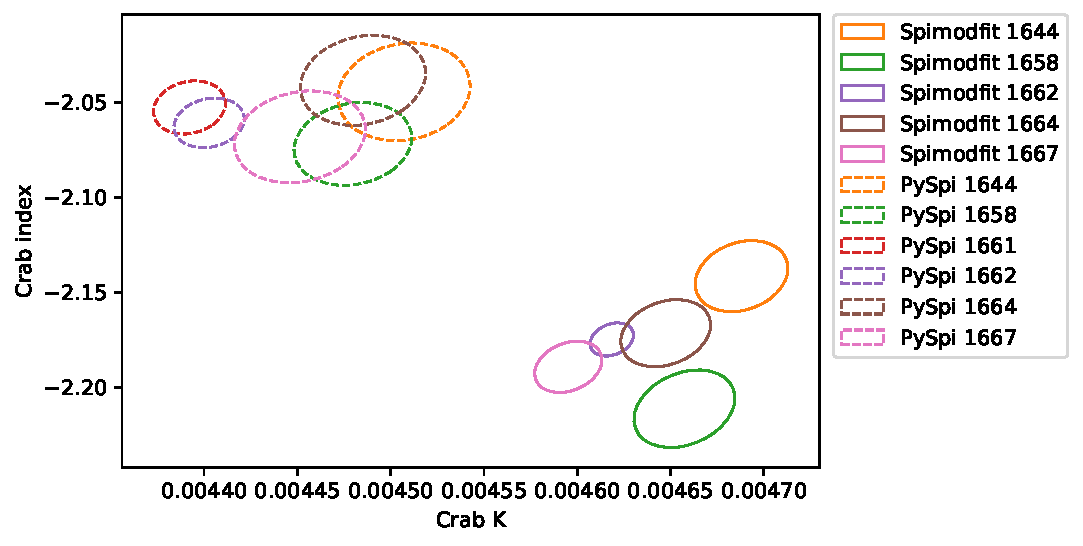
\includegraphics[width=\textwidth]{Images/crab_ps_smf_wo_out.pdf}
    \caption{}
    \label{Crab}
\end{figure}

Figure \ref{Crab} shows one standard deviation confidence intervals of several near SPI Revolutions, as fitted using PySpi and Spimodfit. Revolution 1661 was only fitted using PySpi since spimodfit rejected all SCWs due to "General Expression". The source model is a simple powerlaw 
\begin{equation} \label{powerlaw}
    f(x) = K \frac{x}{piv}^{index}
\end{equation}
where $K$, measured in $\text{keV}^{-1}\text{s}^{-1}\text{cm}^{-2}$ is the differential flux at the pivot value $piv=40$keV, $x$ is the photon energy in keV, and $index$ is the index of the powerlaw.

Both methods used the same energy range of 20-81.5keV, although it is worth pointing out that they use independent algorithms to select which SCWs are used in the fit. PySpi used a cluster size of two. 

Although the two methods obtain different values for the index and normalization, we see comparable sizes of uncertainties as well as similar levels of compactness within the values from different revolutions. 

The data used by PySpi was also subjected to a Posterior Predictive Check (PPC) analysis, allowing for revolution pairs that did not match the source model to be manually removed. This substantially improved the consistency of the fits.

\section{Results: Simulated Source} \label{Sec: Sim Source}
The downside to fitting a real astronomical object such as the Crab nebula is that one can never be exactly sure what the true source parameter values should be. This is why it can be advantageous to simulate a source, feed the simulated data back into the fit, and compare the produced source parameters to the now known true values.

However, not only a simulated source is required, but a background spectrum as well. There are different approaches one may take to realize this:

\begin{enumerate}
    \item \label{step bkg}Choose a data set to use as background. This can be done with real data, in this case a single SPI revolution. For this to work well, there should be as few bright sources within the field of view as possible, since these will interfere with the fit if not included in the source model. This step was also performed using the Spimodfit background spectrum, as described in section \ref{spimodfit bkg}. Alternatively, one can also use a constant background spectrum for all SCWs. This may be realized by choosing one SCW and duplicating its counts to all other SCWs. The counts have to be  redistributed according to a Poisson distribution and the lifetimes of the other SCWs has to be adjusted as well. 
    
    \item Define spectrum of the source to be simulated, as well as position. In this case powerlaws as shown in equation \ref{powerlaw} are used, and the position of the sources is chosen to be central to as many SCWs in the revolution as possible.
    
    \item Use the SPI Instrument Response Function (IRF) to calculate the expected source count rates in each energy bin in each detector for each SCW. Multiply these by the respective lifetimes (effectively the active measuring time) of the detectors in the SCWs, and finally draw a sample of a Poisson distribution with the respective means to attain the measured counts of the simulated source for each energy bin in each detector in each SCW.
    
    \item These source count rates are then added to the background spectrum to acquire the total counts.
\end{enumerate}

This dataset can then be used to fit the simulated source with both PySpi and Spimodfit. When using real data in step \ref{step bkg} this method produces a very realistic background, which in some cases it may be too realistic by including unwanted sources in the field of view that interfere with the fit. This is why it can be beneficial to use the Spimodfit background spectrum or a constant background spectrum instead. The results of this for revolutions 0374 and 1380 are shown in figures \ref{0374 sim source} and \ref{1380 sim source}. Spimodfit was not given the data with a constant background spectrum, since its approach to modelling the background does not allow it to deal with arbitrary spectra. 

\begin{figure}[h]
    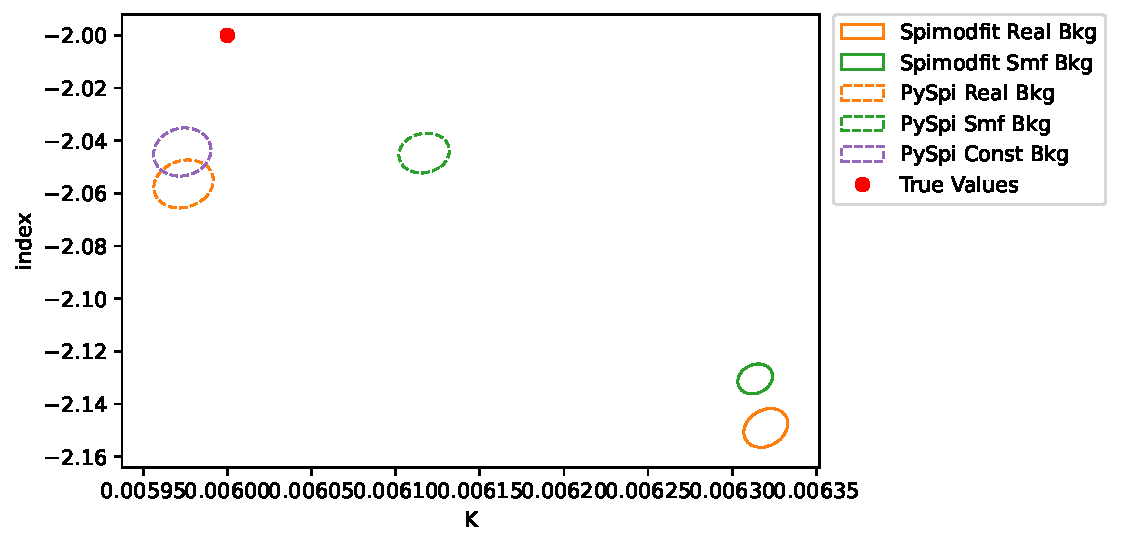
\includegraphics[width=\textwidth]{Images/0374_sim_source.pdf}
    \caption{Simulated Powerlaw source with $K=0.006\text{keV}^{-1}\text{s}^{-1}\text{cm}^{-2}$, $piv=40\text{keV}$, and $index=-2$ for the different methods of generating a background spectrum fitted using PySpi and Spimodfit. This is based on revolution 0374 with the equatorial coordinates of the source at $RA=10, DEC=-40$. As always, the ellipses show the confidence intervals of one standard deviation.}
    \label{0374 sim source}
\end{figure}

\begin{figure}[h]
    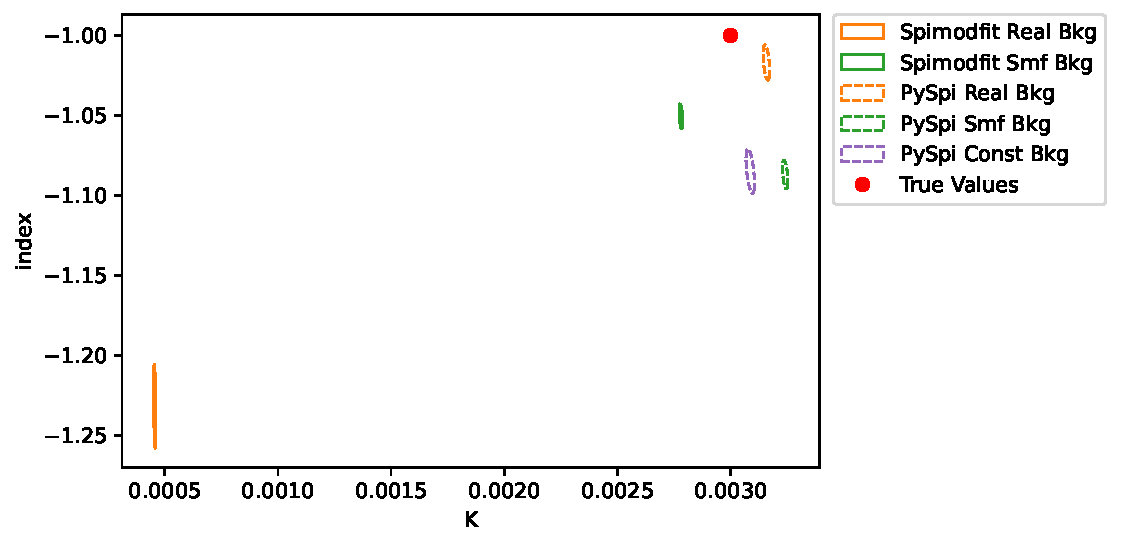
\includegraphics[width=\textwidth]{Images/1380_sim_source.pdf}
    \caption{Simulated Powerlaw source with $K=0.003\text{keV}^{-1}\text{s}^{-1}\text{cm}^{-2}$, $piv=40\text{keV}$, and $index=-1$ for the different methods of generating a background spectrum fitted using PySpi and Spimodfit. This is based on revolution 1380 with the equatorial coordinates of the source at $RA=155, DEC=75$.}
    \label{1380 sim source}
\end{figure}

In general we see PySpi consistently perform better than Spimodfit. A couple of curious results stand out. One is that PySpi performs consistently worse with the Spimodfit background spectrum. In theory, one might not expect this since the Spimodfit background spectrum should not include any point sources in SPIs field of view, so that the fundamental assumption of constant background in SCW clusters should be well met. Another curiosity is that the effect of using Spimodfit with the data produced using the Spimodfit background spectrum has inconsistent results. For revolution 0374 this makes almost no difference to using the real data as background, where as in revolution 1380 the results improve dramatically. Finally, it is very curious how PySpi with a constant background spectrum does not perform as well as one might expect, since the fundamental assumption of constant background is perfectly met. This demonstrates systematic inaccuracies with the PySpi approach to fitting, which are further explored in section \ref{sec: pure sim}.

\begin{figure}[h]
    \centering
    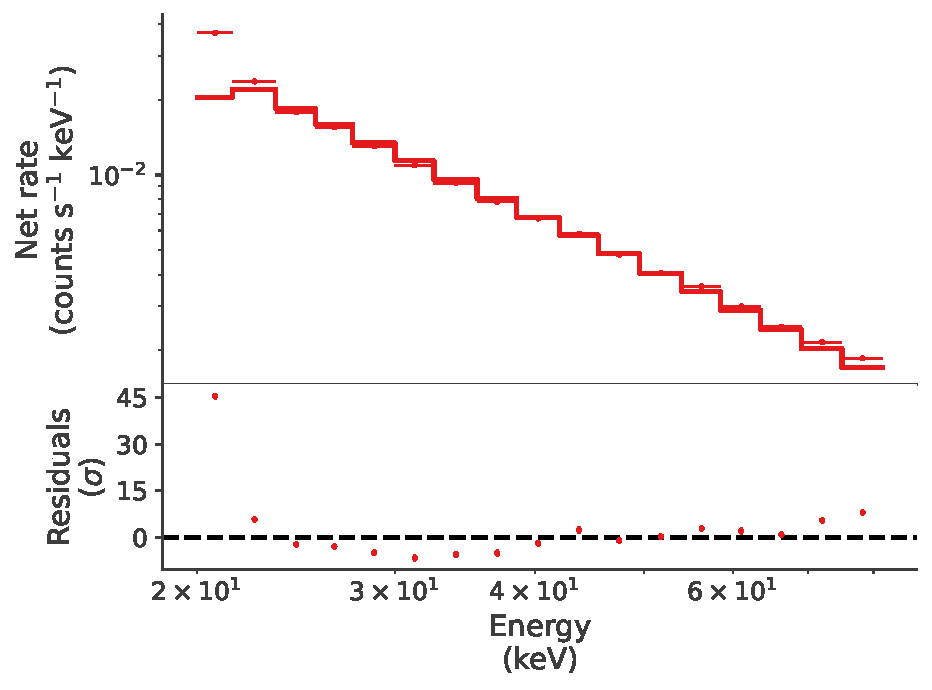
\includegraphics[width=0.7\textwidth]{Images/smf_spec_0374_sim_source.pdf}
    \caption{Spimodfit spectrum and source model for revolution 0374 using the simulated source and the real background spectrum.}
    \label{smf_spec_0374}
\end{figure}

\begin{figure}[h]
    \centering
    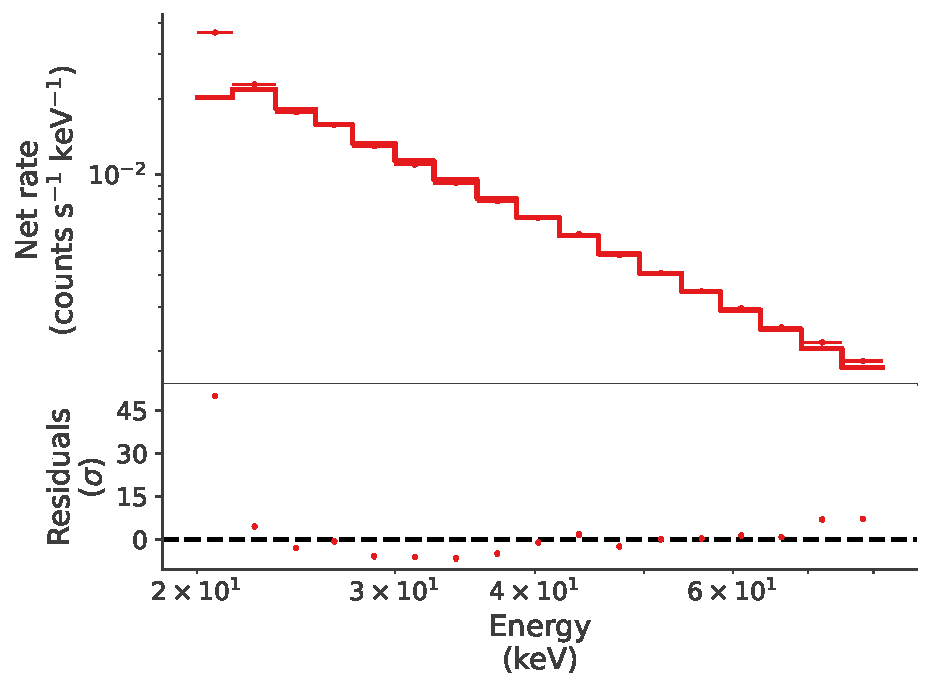
\includegraphics[width=0.7\textwidth]{Images/smf_spec_0374_sim_source_smf_bkg.pdf}
    \caption{Spimodfit spectrum and source model for revolution 0374 using the simulated source and the spimodfit generated background spectrum.}
    \label{smf_spec_0374_smf_bkg}
\end{figure}

\begin{figure}[h]
    \centering
    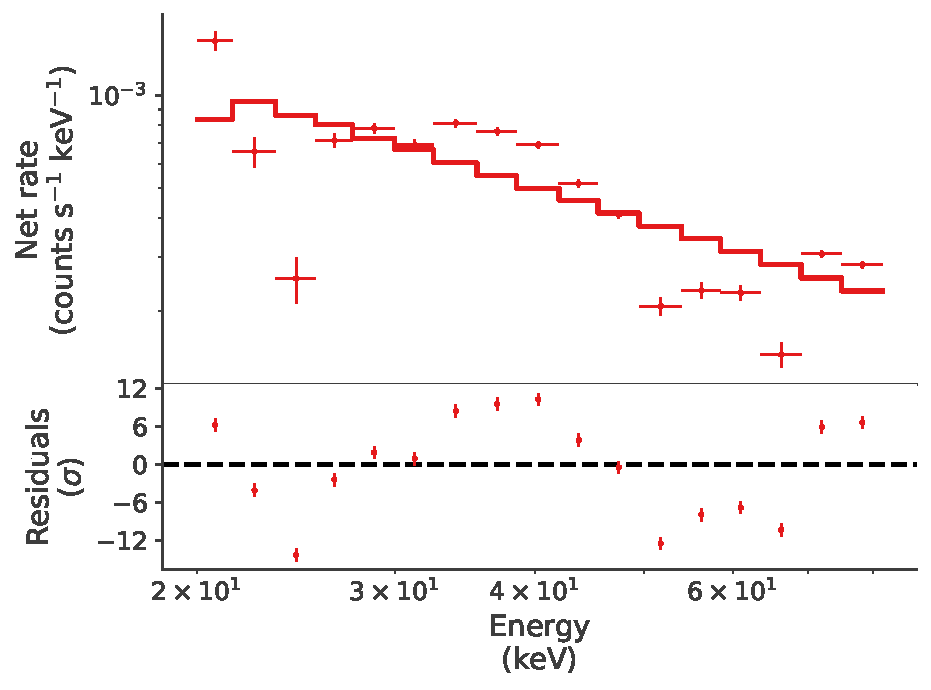
\includegraphics[width=0.7\textwidth]{Images/smf_spec_1380_sim_source.pdf}
    \caption{Spimodfit spectrum and source model for revolution 1380 using the simulated source and the real background spectrum.}
    \label{smf_spec_1380}
\end{figure}

\begin{figure}[h]
    \centering
    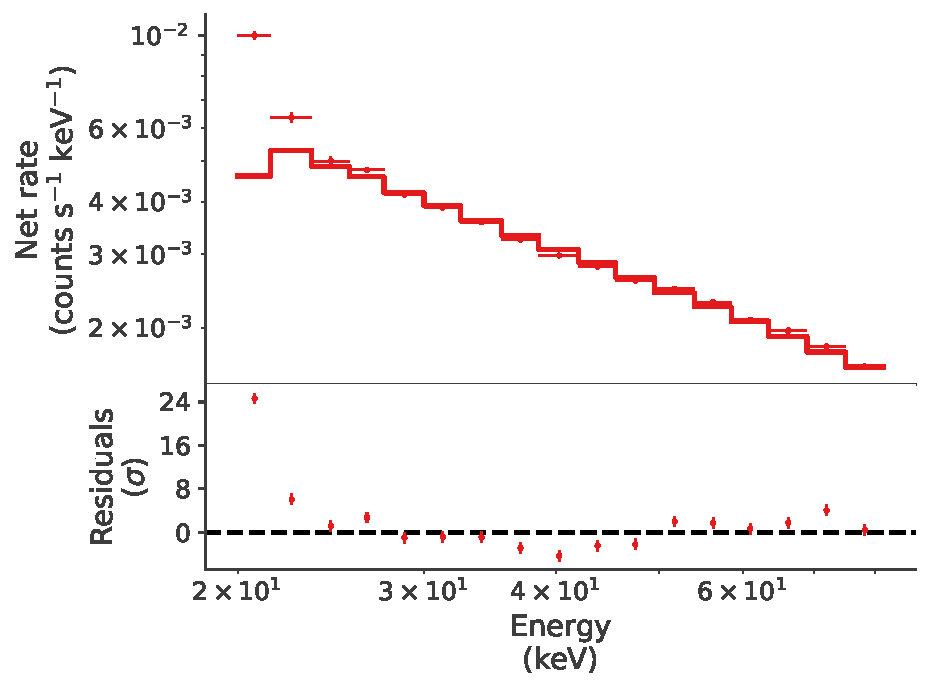
\includegraphics[width=0.7\textwidth]{Images/smf_spec_1380_sim_source_smf_bkg.pdf}
    \caption{Spimodfit spectrum and source model for revolution 1380 using the simulated source and the spimodfit generated background spectrum.}
    \label{smf_spec_1380_smf_bkg}
\end{figure}


Finally, the count and source model spectra produced by the Spimodfit fits are shown in figures \ref{smf_spec_0374} to \ref{smf_spec_1380_smf_bkg}. Two possible signs of errors are that the first energy bin is always significantly higher than predicted by the source model, and that the uncertainties for revolution 1380 with real background data are very high.

\section{Background Analysis}



\begin{figure}[h]
    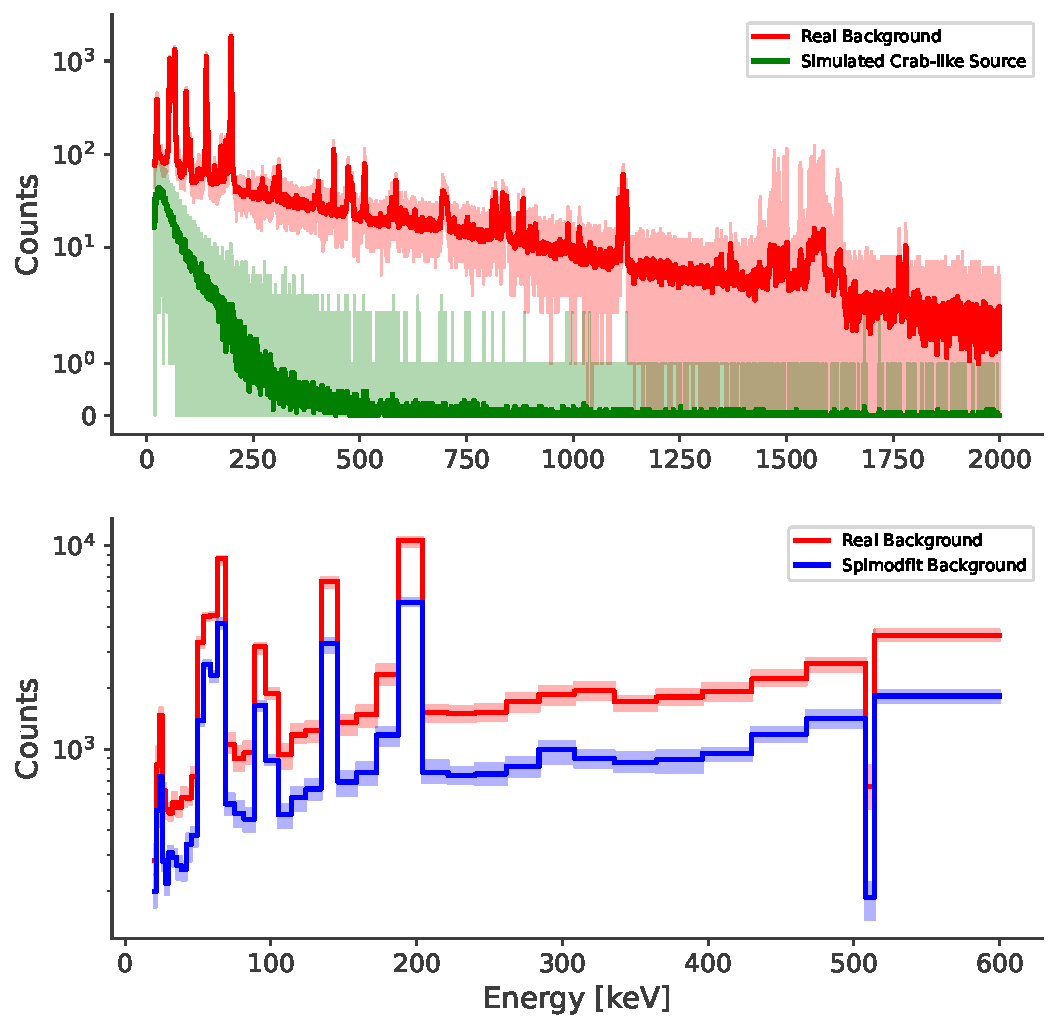
\includegraphics[width=\textwidth]{Images/background.pdf}
    \caption{Background spectrum of SCW 03740002 in comparison to count rates from a simulated source with a powerlaw spectrum similar to that of the Crab nebula. In the bottom plot, the spectrum is rebinned so that it may be compared to the spimodfit background spectrum of the same SCW. The shaded areas show the range over all detectors, whereas the solid line shows the mean over all detectors.}
    \label{plt bkg spec}
\end{figure}

The counts from SCW 03740002 are used very often as an example background spectrum, and duplicated to other SCWs in the revolution for a constant background. Hence, it can be beneficial to visualize this spectrum, as was done in figure \ref{plt bkg spec}. Two things worth noting are that the counts from the simulated Crab-like source are significantly lower than those from the background, especially at higher energies, and that the Spimodfit background spectrum, although very similar in shape, is consistently lower than the real background by a roughly constant factor.

\begin{figure}[h]
    \centering
    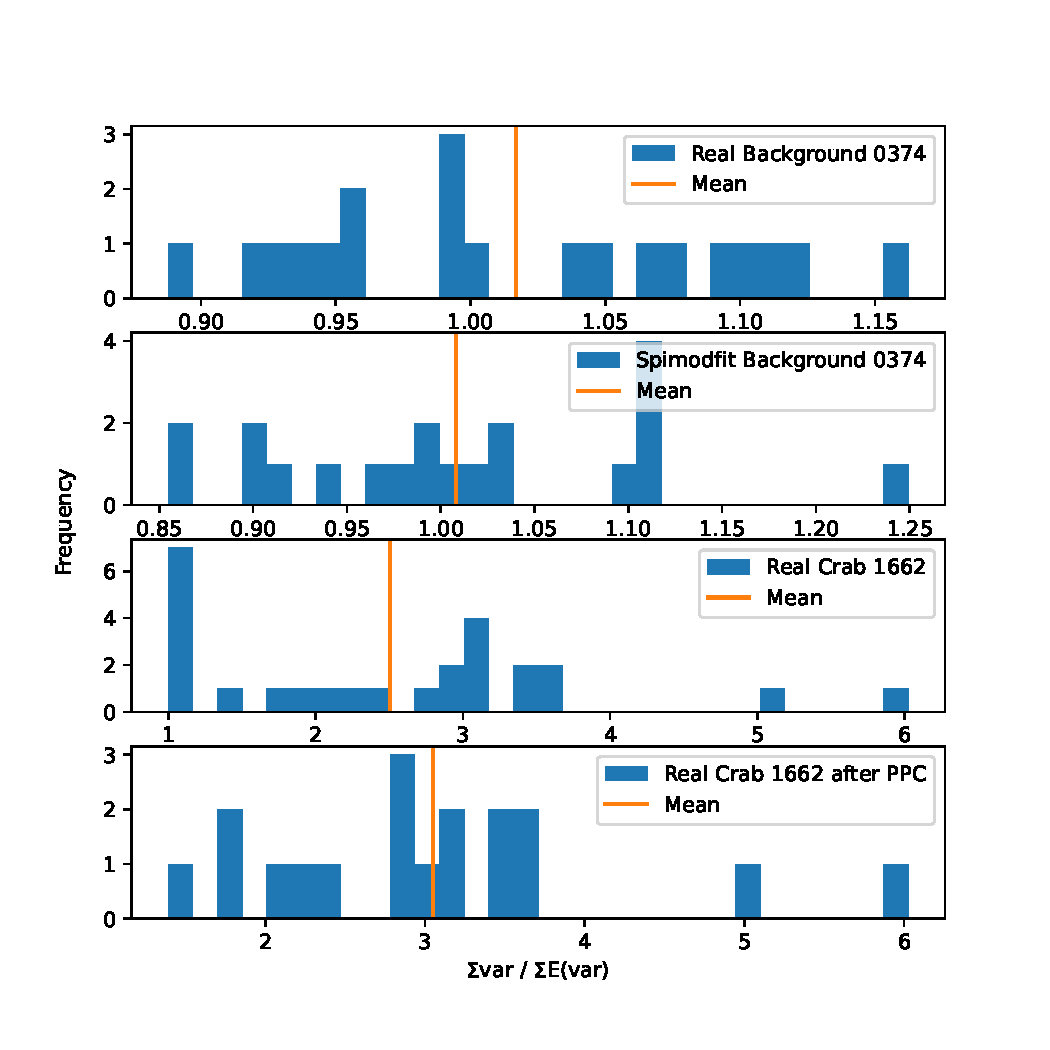
\includegraphics[width=0.9\textwidth]{Images/background_variance.pdf}
    \caption{A histogram of the ratio of the variances to the expected variances based of the SCW clusters for different data sets. (see text)}
    \label{plt bkg var}
\end{figure}

While we are analyzing data spectra that we consider to be background-like (i.e. no point-like source in SPIs field of view), there is a very insightful statistical test we can do. After pairing up SCWs into clusters within a SPI revolution, we can calculate the variance of the counts in each energy bin of each detector of each SCW cluster, and then compare this to the variance we would expect if the two counts were Poisson sampled based on a common underlying background count-rate. The definition of the Bessel corrected variance of the two counts is standard, and the expected variance is also relatively straightforward to compute given the fact that variances of independent distributions add together:

\begin{equation}
    E(var) = (rt_1 - m)^2 + (rt_2 - m)^2 + \frac{r(t_1+t_2)}{2}
\end{equation}

where $r=\frac{C_1+C_2}{t_1+t_2}$ is the average count-rate in both energy bins, $m=\frac{C_1+C_2}{2}$ is the average number of counts, and $t_1$ and $t_2$ are the lifetimes of the respective SCWs. We may then sum the variance and expected variance over all energy bins and all detectors for each cluster of SCWs and take their ratio to get an estimate of how well the fundamental assumption of a constant background count-rate within SCW clusters is met. A ratio $var / E(var)$ around 1 means that the variances between the two SCWs are entirely explained by Poisson sampling with a common count-rate, in comparison to a ratio larger than 1 indicating a source is in SPIs field of view, hence non-common count-rates for identical energy bins in the clustered SCWs.

This was plotted in figure \ref{plt bkg var} for the real data from revolution 0374 and the Spimodfit generated background spectrum for revolution 0374. We see that both are closely distributed around 1, meaning that the fundamental assumption of constant background rates within SCW clusters is well met, both within the real data and the spimodfit generated background. 

Additionally, the same analysis was performed on revolution 1662, featuring many SCWs with the Crab Nebula within 10 degrees of the center of SPIs field of view. As expected, we see that the ratio of the variances is now considerably higher. Curiously, there are still several clusters with a ratio close to 1, implying that there are no visible sources in SPIs field of view. Since the Crab nebula is always within 10 degrees of the field of view, this is impossible. It is unclear what happened in these SCW clusters, but whatever the cause, any sources are completely drowned out. A PPC analysis was conducted on this revolution, with notable outlier SCW clusters being removed from the fit. As expected, this removes exactly those SCW clusters with a variance ratio close to 1. This highlights the importance of performing a PPC analysis when using PySpi.

\section{Results: Pure Simulation} \label{sec: pure sim}
Before we can really draw any conclusions from PySpi fits, we should further observe how accurate the results of PySpi fits are under different conditions. To do this, we once again use the count spectrum from SCW 03740002 as background and duplicate it to others SCWs in the revolution. Different sources are simulated in the following subsections, but the most commonly used source is a powerlaw with the parameters are $K=0.0001\text{keV}^{-1}\text{s}^{-1}\text{cm}^{-2}$, $piv=200\text{keV}$, and $index=-2$, which produces a similar spectrum to the Crab nebula. This revolution contains 42 suitable SCWs for fitting the simulated source at equatorial coordinates $RA=10, DEC=-40$. To measure the accuracy of a fit we shall use the Mahalanobis distance:

\begin{equation}
    d_M = \sqrt{(\vec{V}_F - \vec{V}_T)^TS^{-1}(\vec{V}_F-\vec{V}_T)}
\end{equation}

which tells us the number of standard deviations the fitted source values $\vec{V}_F$ are away from the true source values $\vec{V}_T$, where $S$ is the covariance matrix. Whereas sections \ref{Sec: Crab} and \ref{Sec: Sim Source} used an energy range of 20-81.5keV, this section uses the full energy range of 18-2000keV unless otherwise specified.

\subsection{Consistency}

\begin{figure}[h]
    \centering
    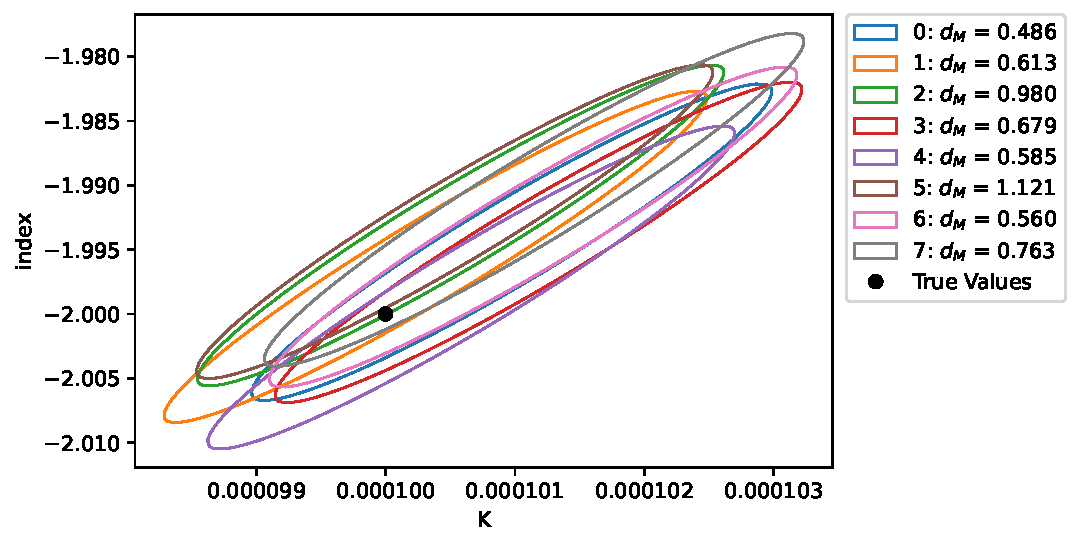
\includegraphics[width=\textwidth]{Images/t_identical_sim_source_sb.pdf}
    \caption{Repeated fits for identical datasets.}
    \label{fig ident}
\end{figure}

The first test is how consistent the fitting is with exactly identical inputs. The results are shown in figure \ref{fig ident}, where the same source is fitted 8 times. We see that the results are actually very consistent, with all of the $1\sigma$ confidence intervals overlapping with each other, and $d_M<1$ for nearly all fits. This result is actually surprisingly good. As we shall see in the following subsections, this exact same source and background will also produce worse fits. A possible explanation is that the count spectra are regenerated for each subsection, meaning that every single Poisson sample is redrawn. This may lead to some datasets for which the fit works better than others. 

\FloatBarrier

\subsubsection{Dynamic Binning}

\begin{figure}[h]
    \centering
    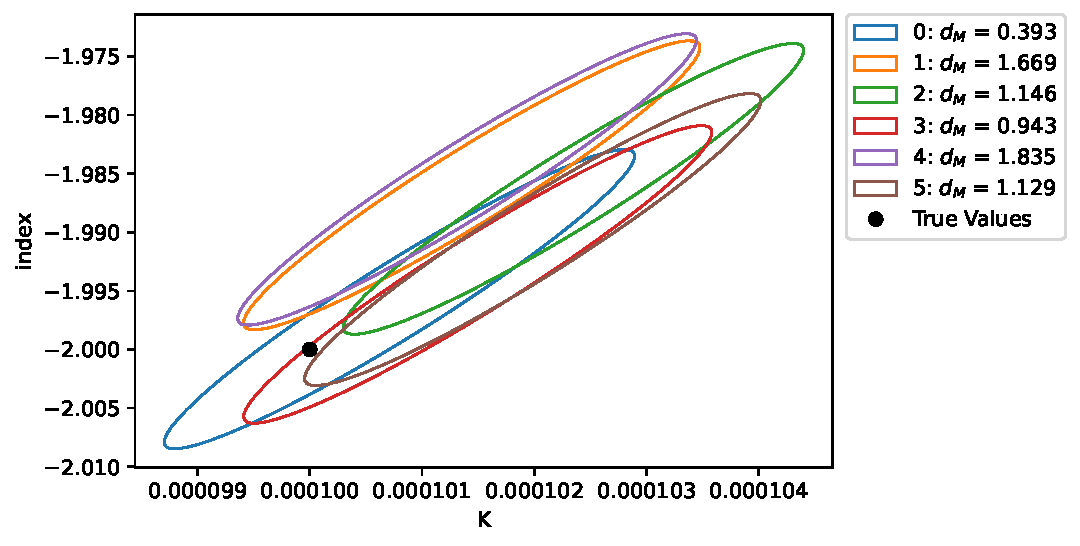
\includegraphics[width=\textwidth]{Images/identical_sim_source_db.pdf}
    \caption{Repeated fits for identical datasets using dynamic binning.}
    \label{fig ident db}
\end{figure}

For most fits, the count spectra are binned into exactly 125 energy bins, spaced semi-logarithmically, which are identical between all SCWs. Another way of binning the data is to use a dynamic binning algorithm, which bins each SCW cluster independently so that the minimum amount of counts is higher than some predetermined value, 50 in this case. A maximum number of bins of 120 was also implemented, since using too many energy bins has a negative effect on computational performance. With this different binning algorithm, we may repeat the same fit on the same data as figure \ref{fig ident}, the results of which are shown in figure \ref{fig ident db}. Strangely, this different binning method seems slightly less consistent than using the exact same energy bins for all SCW clusters. 

\FloatBarrier

\subsection{Different Powerlaws}

\begin{figure}[h]
    \centering
    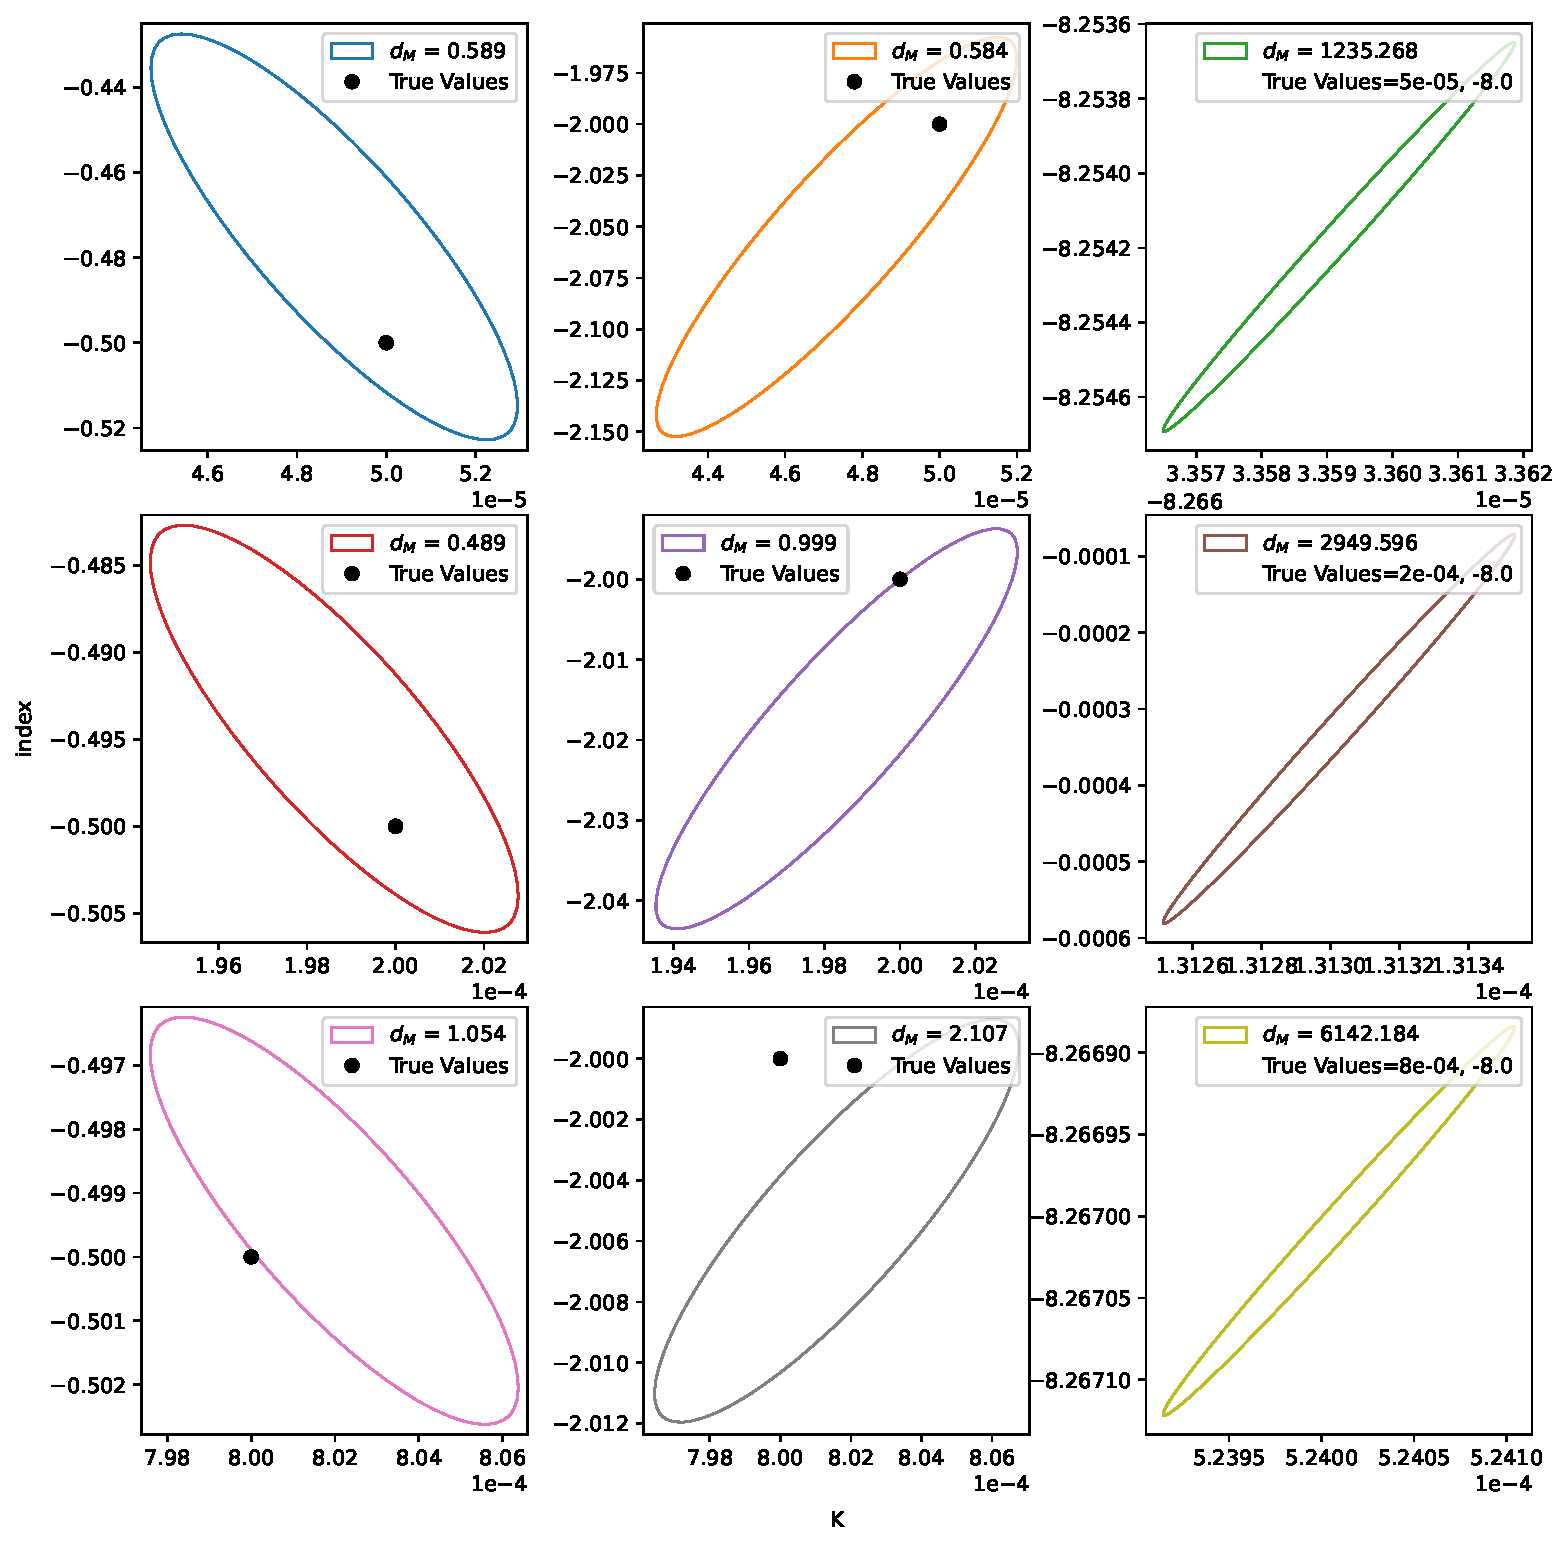
\includegraphics[width=\textwidth]{Images/index_k.pdf}
    \caption{The results of fitting different powerlaws sources. The right column of plots does not show the true values since they are too far away and instead includes the values in the legend.}
    \label{fig index k}
\end{figure}

Another important test is how well the fit works for powerlaws with different parameters. Figure \ref{fig index k} shows the fit results for three different powerlaw indices and three different powerlaw normalizations around a pivot value $piv=100$keV. As one might expect, the fit results have the smallest absolute distance to the true values for bright powerlaws with small indices (in terms of absolute value), since these produce a meaningful amount of counts over the largest range of energies. Surprising is however, that the dimmer sources tend to be fewer standard deviations away from the true values due to their higher uncertainties, and that the fits for powerlaws with the large $index=-8$ fail completely with small uncertainties despite poor accuracies.


\subsection{A Second Source}

\begin{figure}[h]
    \centering
    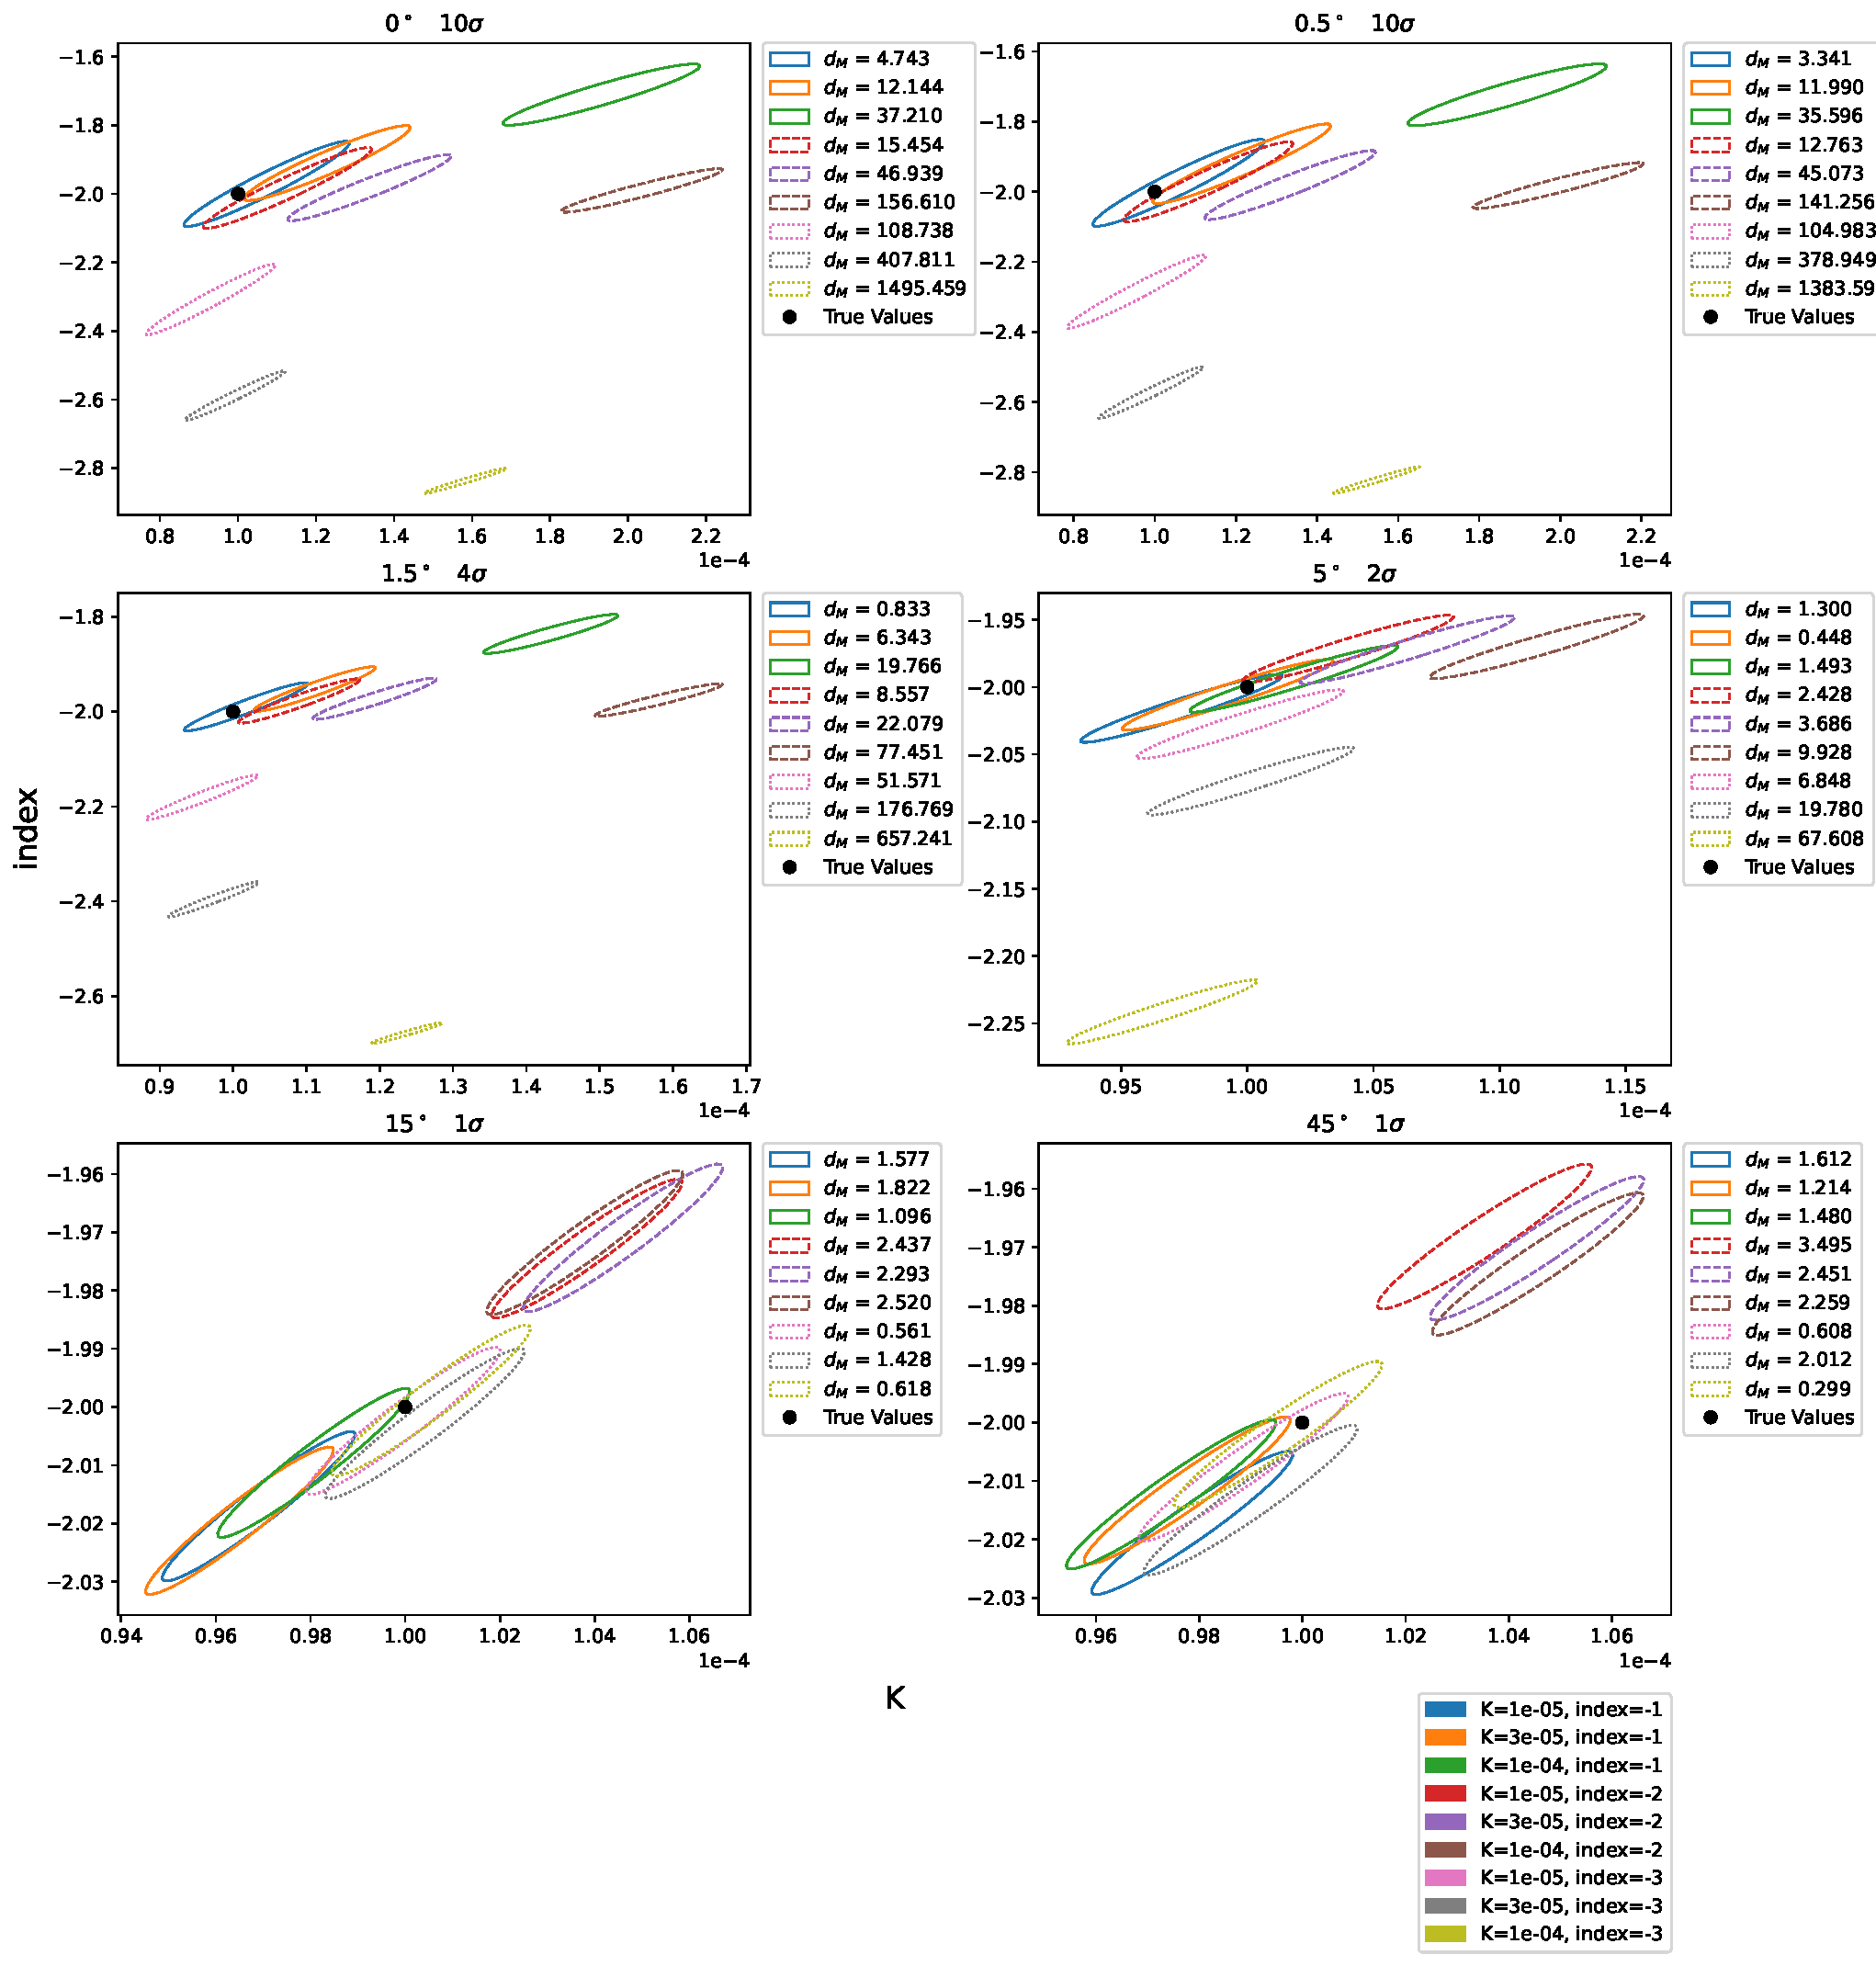
\includegraphics[width=\textwidth]{Images/sec_source.pdf}
    \caption{The effects of a second source, which is not included in the source model of the fit, on the quality of the fit for the primary source. The different plots show results for different angular distances between the two sources, as stated in the respective titles. The titles further show the amount of standard deviations illustrated by the ellipses. Finally, see the legend at the bottom right for the powerlaw parameters of the second source. All powerlaws are normalized at $piv=200$keV.}
    \label{fig sec source}
\end{figure}

In practical applications there are almost always going to be additional sources within SPI's field of view that are not considered in the source model. In order to judge the severity of this, we shall simulate a second source within SPI's field of view (not included in the source model) to observe to ramifications of the fit on the primary source, as is shown in figure \ref{fig sec source}. 

When the two sources are close to each other, the normalization and index shift in accordance to the second source as expected. At 5 degrees apart most fits start to achieve a decent level of quality, and at 15 degrees or more the impact is negligible. The impact is largest when the second source has a large (on an absolute scale) index. One might be inclined to conclude that the second source has significant impact even up to 45 degrees separation, but one should note that Poisson samples used in the background spectra are only redrawn once for every index of the second source. In light of all other results shown here, this seems like the more plausible explanation for the deviations at large separations. 

\FloatBarrier

\subsection{Energy Range}

\begin{figure}[h]
    \centering
    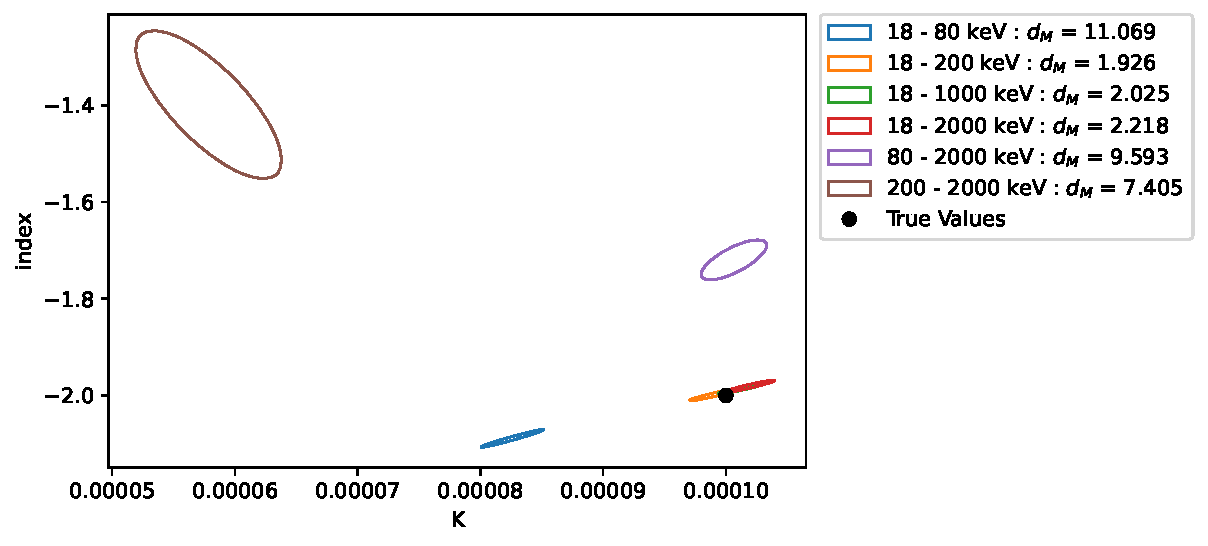
\includegraphics[width=\textwidth]{Images/energy_ranges.pdf}
    \caption{The same dataset fitted using different energy ranges, as shown in the legend.}
    \label{fig energy range}
\end{figure}

Figure \ref{fig energy range} shows the same fit conducted using different energy ranges of the data. We see that the energy range 18-200keV is absolutely crucial for the fit to work well. Since figure \ref{plt bkg spec} shows that this is where the majority of relevant source counts occur for this kind of source, this is not very surprising. It can also be used to explain the systematic errors observed in sections \ref{Sec: Crab} and \ref{Sec: Sim Source}, where an energy range of 20-81.5keV was used.

\FloatBarrier

\subsection{Number of Energy Bins}

\begin{figure}[h]
    \centering
    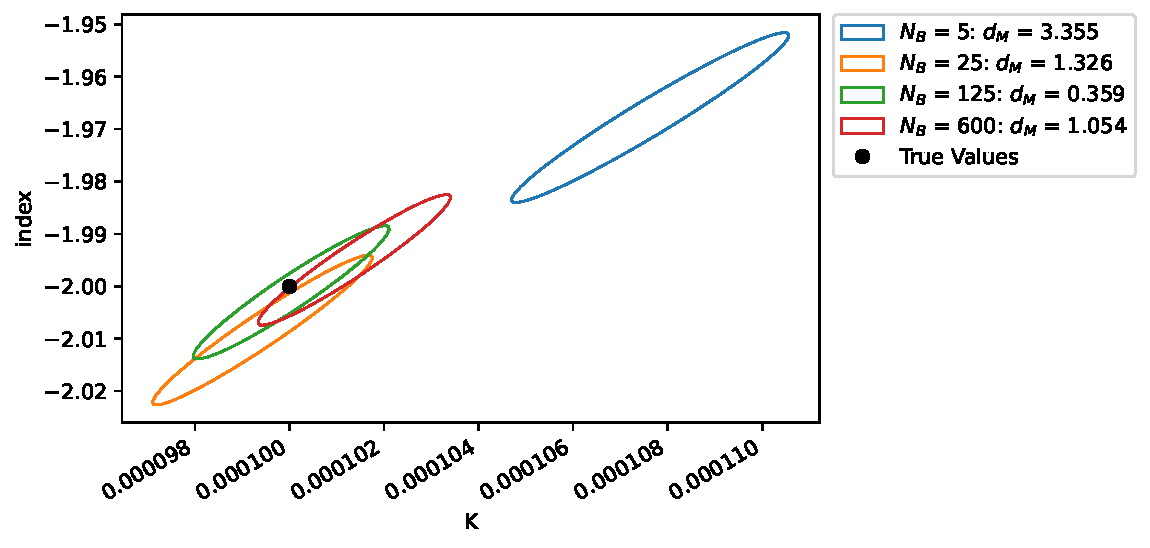
\includegraphics[width=\textwidth]{Images/num_e_bins.pdf}
    \caption{The same data set fitted using a different number of energy bins.}
    \label{fig num bins}
\end{figure}

Seeing how powerlaws do not have fine details that have to be represented with specific energy bins, we would expect the number of energy bins used during the fit to be largely irrelevant. Figure \ref{fig num bins} mostly supports this, with the results for more than 25 energy bins aligning closely. Nonetheless, the result is best for 125 bins, which is convenient since this is also the point where more bins start to have a severe negative impact computational performance.

\FloatBarrier

\subsection{Cluster Size}

\begin{figure}[h]
    \centering
    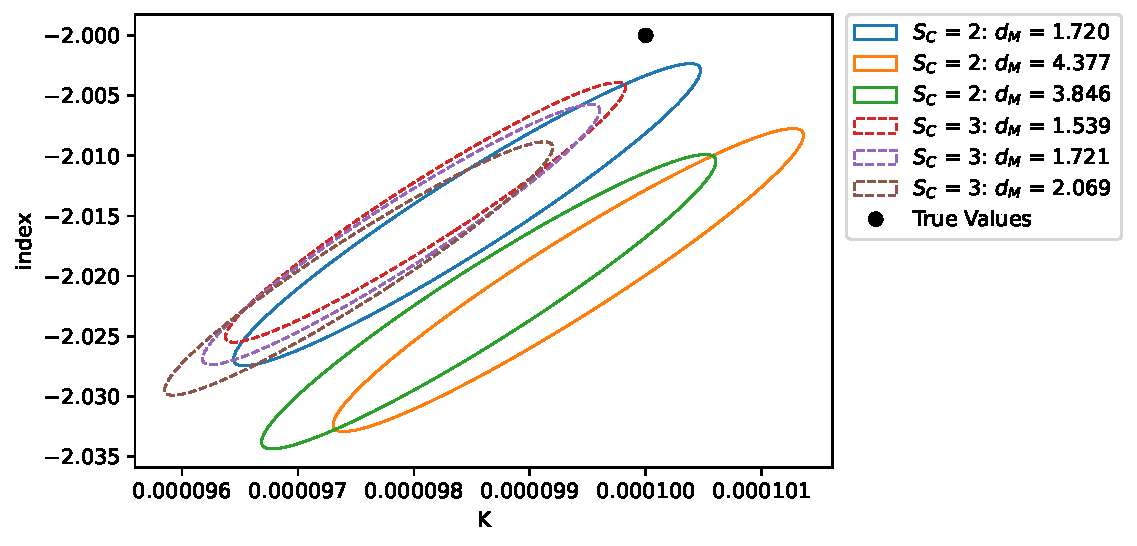
\includegraphics[width=\textwidth]{Images/cluster_sizes.pdf}
    \caption{The same dataset fitted repeatedly using clusters sizes of two and three.}
    \label{fig cluster size}
\end{figure}

So far we have only been using SCW clusters of size two ($S_C=2$) in the fits. Figure \ref{fig cluster size} compares fits using cluster size $S_C=2$ to $S_C=3$. Although the difference is not large, we do see a consistent improvement in both the distance from the true values and the uncertainty size of the fit parameters. Even larger clusters may accentuate this improvement even further. However, in practical applications larger cluster sizes also have downsides. For one, calculating the maximum likelihood background value becomes more complex, and secondly, the the assumption of a constant background count-rate within SCW clusters may become harder to fulfill, since larger cluster sizes necessarily mean larger temporal and spatial differences in the SCWs of the clusters. Further testing is required to see where the optimum lies.

\FloatBarrier

\subsection{Data Scaling}

\begin{figure}[h]
    \centering
    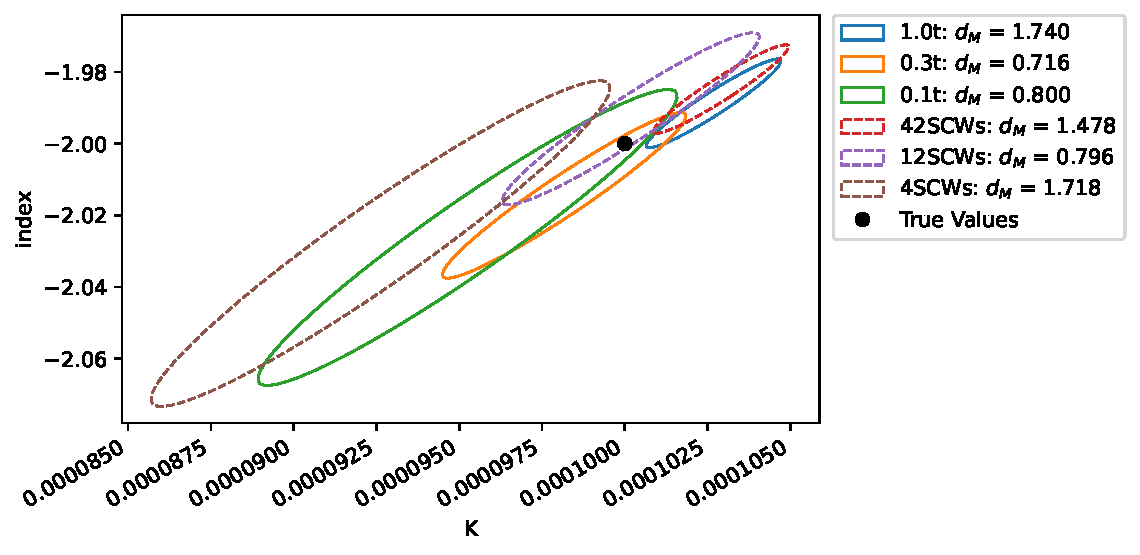
\includegraphics[width=\textwidth]{Images/data_scaling.pdf}
    \caption{Fit results from scaling the amount of lifetime $t$ in each SCW or the amount of SCWs used.}
    \label{fig data scaling}
\end{figure}

Generally speaking, more data will produce better results in any fit. We can test the scaling behavior of the fit quality with the amount of data available to PySpi by scaling the amount of lifetime in each SCW and by scaling the amount of SCWs used in the fit, as shown in figure \ref{fig data scaling}. Unsurprisingly, the fit quality scales very similarly with both of these parameters. The scaling further implies that even larger datasets will produce even smaller uncertainties and errors in the fit. 


\section{PPC Analysis}

List examples of things that can make a SCW bad to justify need for PPC analyis...
Solar Flares,
Supernova / other similar events 

\subsection{Theory}

\subsubsection{General Procedure} \label{PPC general}

A Posterior Predictive Check (PPC) is usually conducted in the following way:

\begin{enumerate}
    \item Fit the data to some model, so that a distribution for the posterior is produced.
    \item \label{Posterior sample} Randomly sample from the posterior.
    \item \label{ppc calc count rates} Using the IRF and the model described by the sampled posterior parameters, calculate the expected count rates in every energy bin of every detector of every SCW.
    \item \label{ppc poisson sample} Taking into consideration the lifetime of each detector in every SCW, draw a sample from the Poisson distribution that describes the measured counts in each bin.
    \item Repeat from step \ref{Posterior sample} until a sufficiently detailed distribution of expected counts for every bin is achieved.
\end{enumerate}

This PPC count distribution can the be used in a variety of ways, such as simply plotting the distribution of expected counts next the actually measured counts. Perhaps one of the most useful applications is the Cumulative Distribution Function (CDF), where one sorts the PPC count distribution of each bin according to size, and the finds the percentile in which the number actually measured counts falls. If the model described using the posterior values perfectly matches reality one would expect values evenly distributed between 0 and 1, whereas if the model is not a good representation of reality the distribution will not be even. 

In the context of PySpi it makes sense to organize these CDF values into a histogram for every SCW used in the fit. This way individual SCWs for which the model does not match the measured data can be identified and excluded from a repeated fit with hopefully better results.

\subsubsection{PySpi Application}
As an attentive reader may have already identified, there is a problem with using the procedure previously described in section \ref{PPC general} for PySpi: the model used the fit (see section \ref{General Procedure}) is purely a source model, i.e. it tells us nothing about the background count rates. This is a problem because it means we cannot calculate the expected count rates in step \ref{ppc calc count rates} of section \ref{PPC general} without being able to describe the background.

The only way to circumvent this problem is with the same approach used in section \ref{General Procedure} of the actual fit. After having calculated the expected source count rates for a sample of the posterior we can use the actually measured counts to calculate the maximum likelihood background count rates and continue our analysis with it.

However, there is a drawback to this solution: in step \ref{ppc poisson sample} of section \ref{PPC general} we can no longer use a simple Poisson distribution to sample expected measured counts from the calculated count rates. This is because we have introduced a bias into our expected count rates by using the actually measured counts in the calculation. For example, if some energy bin has measured a statistically large number of counts (in accordance to the Poisson distribution of the true count rates), then the maximum likelihood background calculated using the actually measured counts will naturally increase with the actually measured counts. This way any statistical outliers are significantly dampened, thus defeating the purpose of conducting the PPC analysis to begin with.

To quantify this bias we will have to do some math. The following equations are applicable to every energy bin for every detector in every SCW cluster. As in section \ref{General Procedure} we will focus on clusters of size 2, although the process is analogous for larger cluster sizes.

For every bin and every SCW there exists a true source count rate $s_1$ and $s_2$ as well as a true background count rate $b$. The source count rates vary between the SCWs of one cluster, whereas the background count rate is constant. If $t_1$ and $t_2$ are the lifetimes of the SCWs, the actually measured counts $b_{1m}, b_{2m}, s_{1m}$ and $s_{2m}$ from the respective sources will be Poisson distributed

\begin{align*}
    B_{1m} &= P(bt_1) \\
    B_{2m} &= P(bt_2) \\
    S_{1m} &= P(s_1t_1) \\
    S_{2m} &= P(s_2t_2)
\end{align*}

so that the total number of measured counts $C_{1m}$ and $C_{2m}$ are simply

\begin{align*}
    C_{1m} &= B_{1m} + S_{1m} \\
    C_{2m} &= B_{2m} + S_{2m}.
\end{align*}

Arriving at an equation for the distributions $C_{1m}$ and $C_{2m}$ is our goal for the PPC analysis. We may assume that true source count rates $s_1$ and $s_2$ equal those predicted by our source model from the posterior samples, since testing that assumption is the whole point of doing the PPC analysis to begin with. The true background count rate $b$, however, remains unknown to us. Instead we can only calculate the maximum likelihood background $b_M$, as described previously. In order to be able to draw samples from the probability distributions $C_{1m}$ and $C_{2m}$ we must relate relate the distributions of the quantities that we do know ($s_1, s_2, t_1, t_2, b_M$) to those that we wish to know ($b$):

\begin{align*}
    B_{d1} &= B_{1m} - b_Mt_1 \\
    B_{d2} &= B_{2m} - b_Mt_2 \\
    S_{d1} &= S_{1m} - s_1t_1 \\
    S_{d2} &= S_{2m} - s_2t_2.
\end{align*}

$B_{d1}$ and $B_{d2}$ tell us the difference between quantities we have readily available ($b_Mt_1$ and $b_Mt_2$) to those directly necessary in the PPC analysis ($B_{1m}$ and $B_{2m}$). This means that if we calculate their variances and approximate the resulting distribution as normal we can directly draw random samples according to the distribution of $B_{1m}$ and $B_{2m}$, without having to know the true background rate $b$. Furthermore, we also have to consider that the distribution of $b_M$, which we utilize in $B_{d1}$ and $B_{d2}$, is correlated with the distribution $S_{1m}$ and $S_{2m}$. Hence, we not only have to calculate the variances of $B_{d1}$ and $B_{d2}$, but also the covariances of $B_{d1}$ with $S_{d1}$ and $B_{d2}$ with $S_{d2}$, respectively. To draw a random sample from $B_{1m}$ and $S_{1m}$ we thus sample from a multivariate normal with mean $\mu$ and covariance matrix $cov$:

\begin{equation*}
    \mu = \begin{pmatrix}
        b_Mt_1 \\ s_1t_1
    \end{pmatrix} 
\end{equation*}
\begin{equation*}
    cov = \begin{bmatrix}
        variance(B_{d1}) & covariance(B_{d1}, S_{d1})\\ covariance(B_{d1}, S_{d1}) & variance(S_{d1})
    \end{bmatrix}
\end{equation*}
Hence: 
\begin{equation*}
    \begin{pmatrix}
        B_{1m} \\ S_{1m}
    \end{pmatrix}
    \sim \mathcal{N}(\mu, cov)
\end{equation*}
This works because we can assume that the expected value of the maximum likelihood background rate is equal to the true background rate: $E(b_M) = b$. Analogous arguments can be made for the second SCW. It is worth noting that approximating the distribution shapes as normal should have negligible impact as long as the number of counts per bin are sufficiently large.

Now that we have understood the motivation, the tricky part is actually calculating these variances.


\end{document}